\chapter{Implementación}
\title{Implementación}
\label{cap:Implementacion}


\section{Red}
\title{Red}

En el sistema a desarrollar, ya se ha manifestado la intención de crear distintos
tipos de dispositivos. También es necesario establecer una comunicación entre ellos,
es decir, una red. A lo largo de las siguientes secciones iremos viendo cómo se
ha implementado.\\

\subsection{Topología}
\title{Topología}
En primer lugar hay que remitirse a los distintos diagramas que se han ido
realizando para explicar la estructura propuesta, como el diagrama de despliegue (figura \ref{fig:diagramadespliegue}).\\

Se observa que todos los nodos (músicos) se comunican, única y exclusivamente, con un nodo central (director).
Es por elo que la topología de nuestra red debe ser una \textbf{topología en estrella}.\\

\subsection{Red inalámbrica de sensores}
\title{Red inalámbrica de sensores}

Para crear la red se va a optar por formar una red inalámbrica de sensores ya que es
el tipo de infraestructura que cumple con las necesidades del sistema a desarrollar.\\

Una red inalámbrica de sensores (\textit{WSN, Wireless Sensor Network}) es aquella formada por un
conjunto de elementos autónomos cuyo objetivo es el de solucionar una tarea utilizando
comunicación inalámbrica. Los nodos que forman la red no disponen de alta capacidad funcional
y tienen un costo energético bajo (siendo posible su alimentación a través de baterías de poca capacidad).\\

\begin{figure}[htb]
\centering
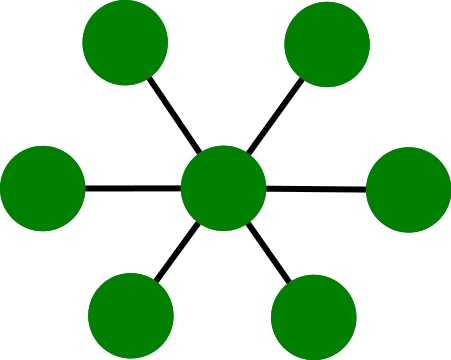
\includegraphics[width=0.8\textwidth]{./imagenes/estrella}
\caption{Topología en estrella} \label{fig:estrella}
\end{figure}

\subsection{Método a utilizar}
\title{Método a utilizar}
Dentro de las \textit{WSN}, podemos elegir entre distintos métodos para realizar la
comunicación entre nuestras motas. Según las necesidades que tenga nuestra red,
utilizaremos uno u otro. Se van a analizar brevemente algunos de los principales:

\begin{description}
  \item[WiFi] \hfill \\
    Basado en el estándar IEEE 802.11. Alta velocidad en transferencia de datos
    (permite adaptación a la velocidad de transmisión) y seguridad en la red pero
    no dispone de mecanismos para ahorrar energía
  \item[Bluetooth] \hfill \\
    Otro estándar de comunicación entre dispositivos. Permite broadcast, una velocidad
    de hasta 24Mbit/s y sus redes son de hasta 8 nodos (uno maestro y siete esclavos).
    En la versión 4 se han introducido métodos para reducir el consumo de energía
  \item[802.15.4] \hfill \\
    Es un estándar propuesto por el IEEE. El ancho de banda es muy pequeño, la latencia
    se sitúa en torno a los 15ms, alcance de entre 10 y 20 metros, permite tener miles
    de nodos en la red, mecanismos para tener un bajísimo consumo de energía y barato
  \item[ZigBee] \hfill \\
    Es un estándar desarrollado sobre 802.15.4, lo que quiere decir que añade capas a la
    propuesta hecha en 802.15.4 (añadiendo algunas funciones)
\end{description}

Todos estos métodos permiten la topología en estrella.\\

Teniendo en cuenta el análisis anterior se concluye que:
\begin{itemize}
  \item WiFi queda descartado: aunque existan redes de sensores que utilicen esta tecnología,
  WiFi no contempla mecanismos para el ahorro de energía. Aunque vaya a ser necesaria una alta velocidad
  (debido a los requisitos temporales del sistema), no hace falta tanta como la que
  proporciona este mecanismo de comunicación (por lo que se vería desperdiciada)
  \item Bluetooth se descarta: a través de la capa de aplicación, algunas implementaciones
  de redes inalámbricas de sensores han conseguido aumentar el número máximo de nodos por red.
  Por otra parte, aunque la versión 4 de Bluetooth esté pensada para economizar el gasto energético,
  este sigue siendo demasiado alto (es algo que cualquier usuario experimenta día a día cuando
  conecta unos auriculares, un manos libres o una smartband a su smartphone, descendiendo el nivel de
  carga de la batería a una velocidad muy alta)
  \item 802.15.4 o ZigBee son la solución: cumplen con casi todos los requisitos.
  El problema que puede presentarse viene dado por las velocidades de transferencia: aunque no
  se necesite realizar grandes traspasos de información, las comunicaciones deben
  hacerse de la manera más rápida posible. Hay que tener en cuenta que ZigBee está construido a partir
  de 802.15.4, lo que significa que la latencia será mayor (habrá que sumar la de 802.15.4 a la que provoquen
  las capas que añade ZigBee). También puede ocurrir que en el canal en el que se estén realizando las comunicaciones
  se esté produciendo otra (en ese caso, la velocidad de transmisión disminuirá)
\end{itemize}

\begin{figure}[htb]
\centering
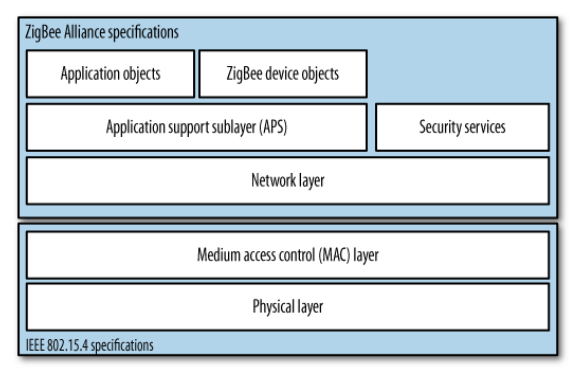
\includegraphics[width=1\textwidth]{./imagenes/zigbeestack}
\caption{ZigBee Stack. Imagen extraída de \cite{faludi} (figura 8.1) } \label{fig:stackzigbee}
\end{figure}

Finalmente se ha elegido trabajar con ZigBee aunque, probablemente, con 802.15.4 sería suficiente (incluso
mejor al tener una menor latencia). El motivo de esta selección viene determinado porque las motas disponibles
en el laboratorio son de tipo ZigBee, no habiendo de la otra variedad.\\

Para ser más específicos, se va a utilizar el modelo “XBee 2mW Wire Antenna - Series 2 (ZigBee Mesh)”, cuya referencia es
“XB24-Z7WIT-004” (ID: OUR XBEE2 e IC: 4214A-XBEE2) y que es la implementación de la compañía “Digi” \cite{productdetaildigi}.


\begin{figure}[htb]
\centering
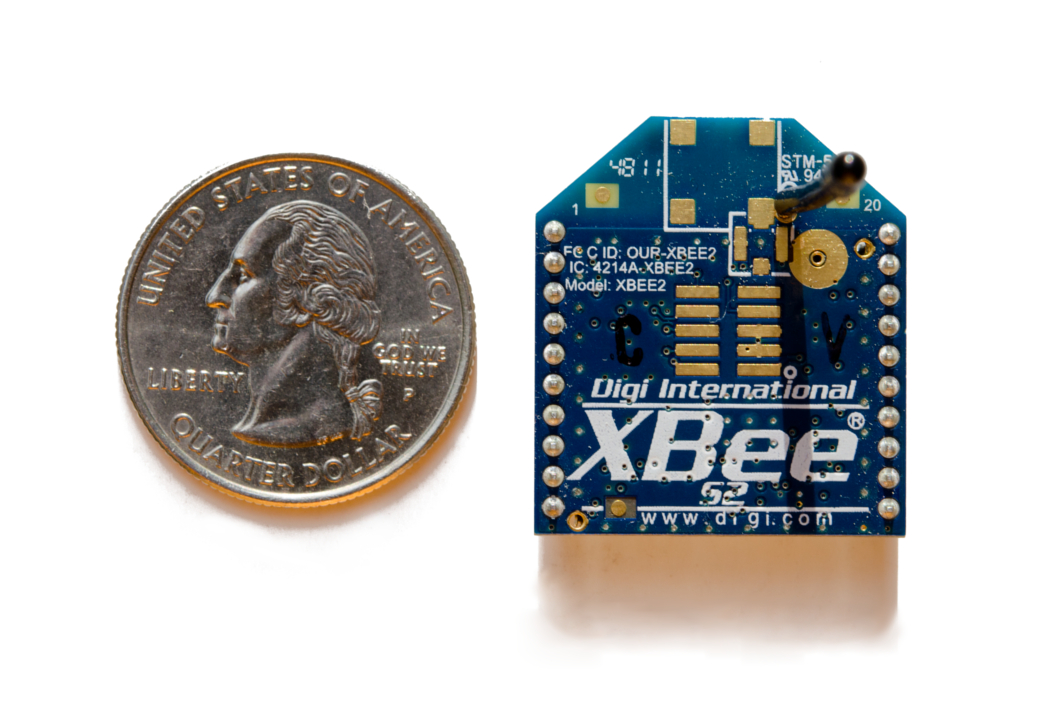
\includegraphics[width=1\textwidth]{./imagenes/xbeequarter}
\caption{Una mota XBee junto a un cuarto de dólar. Imagen extraída de \scriptsize{https://en.wikipedia.org/wiki/XBee} } \label{fig:xbeequarter}
\end{figure}

\begin{figure}[htb]
\centering
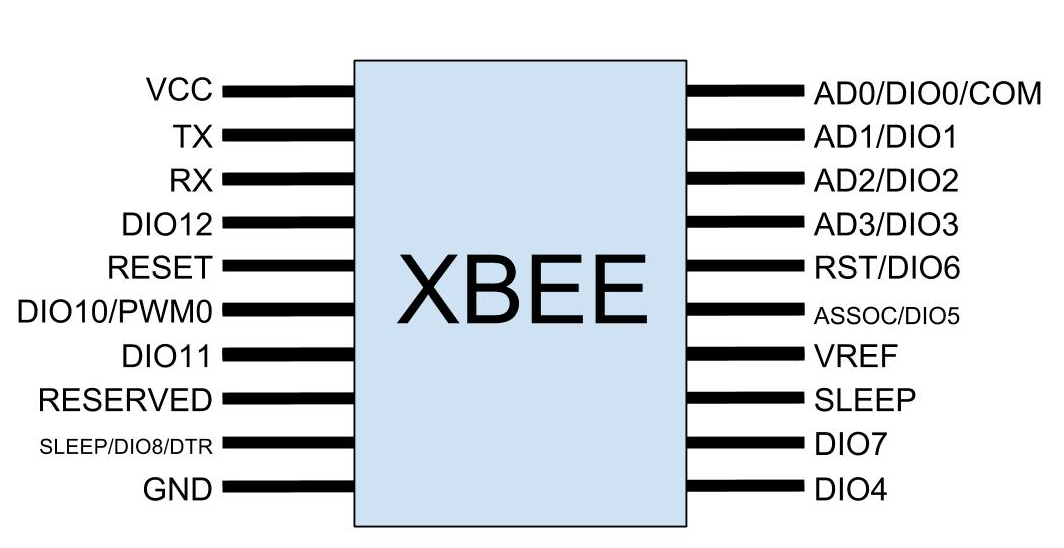
\includegraphics[width=1\textwidth]{./imagenes/xbeepinout}
\caption{XBee PINOUT} \label{fig:xbeepinout}
\end{figure}

En la figura \ref{fig:xbeepinout} podemos ver el esquema de XBee Series 2.

\begin{itemize}
  \item VCC: alimentación
  \item TX: pin de salida de comunicación serial
  \item RX: pin de entrada de comunicación serial
  \item DIO12: entrada o salida digital
  \item Reset: permite resetear el módulo
  \item DIO10/PWM0/RSSI: tiene tres funcionalidades (entrada/salida digital,
    RSSI -”Indicador de Intensidad de la Señal”- o pin de modulación por ancho de pulsos)
  \item DIO11: entrada o salida digital
  \item Reserved: es un pin reservado. No se aconseja conectarlo a nada
  \item SLEEP/DIO8/DTR: también dispone de varias funciones (control de sueño de la mota,
    entrada/salida o señal hardware de handshaking).
  \item GND: tierra
  \item DIO4: entrada o salida digital
  \item DIO7: entrada o salida digital. También puede hacer las funciones de “clear to send”
  \item SLEEP: indicador de sueño. Permite saber si la mota se encuentra durmiendo
    o no (si el estado es alto, se encuentra en funcionamiento)
  \item VFREF: no tiene funcionalidad en este modelo
  \item ASSOC/DIO5: doble función (indicador de pertenencia a red -estado alto si
    está asociada a una red- o entrada/salida digital)
  \item RST/DIO6: doble función (petición de envío o entrada/salida digital)
  \item AD3/DIO3: entrada salida analógica o digital
  \item AD2/DIO2: entrada salida analógica o digital
  \item AD1/DIO1: entrada salida analógica o digital
  \item AD0/DIO0/COM: triple funcionalidad (entrada/salida digital o analógica o puesta en servicio)
\end{itemize}

Sus características técnicas son:
\begin{itemize}
  \item 3.3V @ 40mA
  \item 250kbps Max data rate
  \item 2mW output (+3dBm)
  \item 400ft (120m) range
  \item Built-in antenna
  \item Fully FCC certified
  \item 6 10-bit ADC input pins
  \item 8 digital IO pins
  \item 128-bit encryption
  \item Local or over-air configuration
  \item AT or API command set
\end{itemize}

En este último punto se nos hablan de dos modos de funcionamiento:

\begin{description}
  \item[AT] \hfill \\
    Es el modo transparente. Una vez establecida la configuración (mediante comandos
    que se envían al dispositivo a través de serial), el dispositivo solo es capaz de
    comunicarse con la mota cuya dirección MAC corresponde con la de la configuración
    (también pueden enviarse paquetes a todos los dispositivos en caso que la dirección
    que se haya configurado sea la de broadcast). Esto quiere decir que, en caso que
    deseemos cambiar el destino de nuestras comunicaciones, tendremos que reconfigurar
    la mota (ya sea enviando comandos AT o utilizando algún software que los envíe
    por nosotros) Es el modo más simple de trabajar con XBee.
 \item[API] \hfill \\
    Este modo permite mucho más. Capacita al desarrollador a:
      \begin{itemize}
        \item Obtener RSSI (fortaleza de la señal respecto a otro dispositivo),
        \item Enviar paquetes a múltiples destinos
        \item Recibir paquetes de distintos tipos
        \item Activar funciones de integridad de datos, recibir ACK...
        \item Conocer el estado de la red
      \end{itemize}
\end{description}



\subsection{Modo API}
\title{Modo API}

Mientras que en el modo transparente los caracteres que escribamos en el puerto
serial de XBee serán enviados directamente a la mota destino, en este modo las
comunicaciones se realizan enviando paquetes con una estructura predefinida.\\

Existen dos formas de comunicarse con la mota cuando se encuentra en este modo:
\begin{itemize}
  \item Pines de entrada/salida: en el caso de querer dar una salida, la deberemos preestablecer en la configuración.
  Un pin que se configure en modo entrada, tomará el valor que le llegue y la mota enviará el valor a la mota destino.
  La propia mota genera el paquete y lo envía.
  \item Puerto serial: permite la creación y envío de distintos tipos de paquetes.
  Esto se hace de forma manual, es decir, se precisa de un controlador que escriba los valores en el puerto serial de XBee.
\end{itemize}

Cada paquete que envía (o recibe) un dispositivo XBee, tiene la estructura de la figura \ref{fig:tramaapi}.

\begin{figure}[htb]
\centering
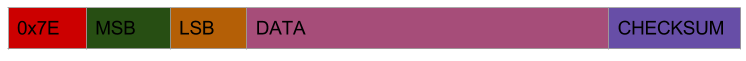
\includegraphics[width=1\textwidth]{./imagenes/tramaapi}
\caption{Paquete XBee en modo API} \label{fig:tramaapi}
\end{figure}

\begin{itemize}
  \item 0x7E: comienzo de la trama
  \item MSB: byte más significativo para la traza
  \item LSB: byte menos significativo para la traza
  \item DATA: puede incluir varias cosas, como el tipo de comando API o AT que se está enviando, parámetros… (para conocer más, )
  \item CHECKSUM: checksum de la trama
\end{itemize}

Para generar estas tramas utilizaremos una biblioteca open source que se encuentra en GitHub (\cite{libraryArduinoXBee}).
Gracias a ella, no tendremos que preocuparnos de generar los distintos elementos del paquete
(como el delimitador de comienzo o el cálculo del checksum).\\

Para conocer más sobre el modo API, el lector puede consultar el capítulo 5 (\textit{API and a Sensor Network}) de \cite{faludi}.\\

\subsection{XCTU: el software para manipular las motas}
\title{XCTU: el software para manipular las motas}
Este software es distribuido gratuitamente por Digi \cite{licenciaXCTU} y se puede descargar desde la página oficial
de dicha empresa.

Para conectar XBee a nuestro ordenador, debemos conectar las patillas de XBee del puerto serial a un
FTDI (por ejemplo) y con una conexión serial o USB, a nuestro ordenador. Otra posibilidad es obtener
una placa ``XBee Explorer" como la de la figura \ref{fig:xbeeexplorer}.


\begin{figure}[htb]
\centering
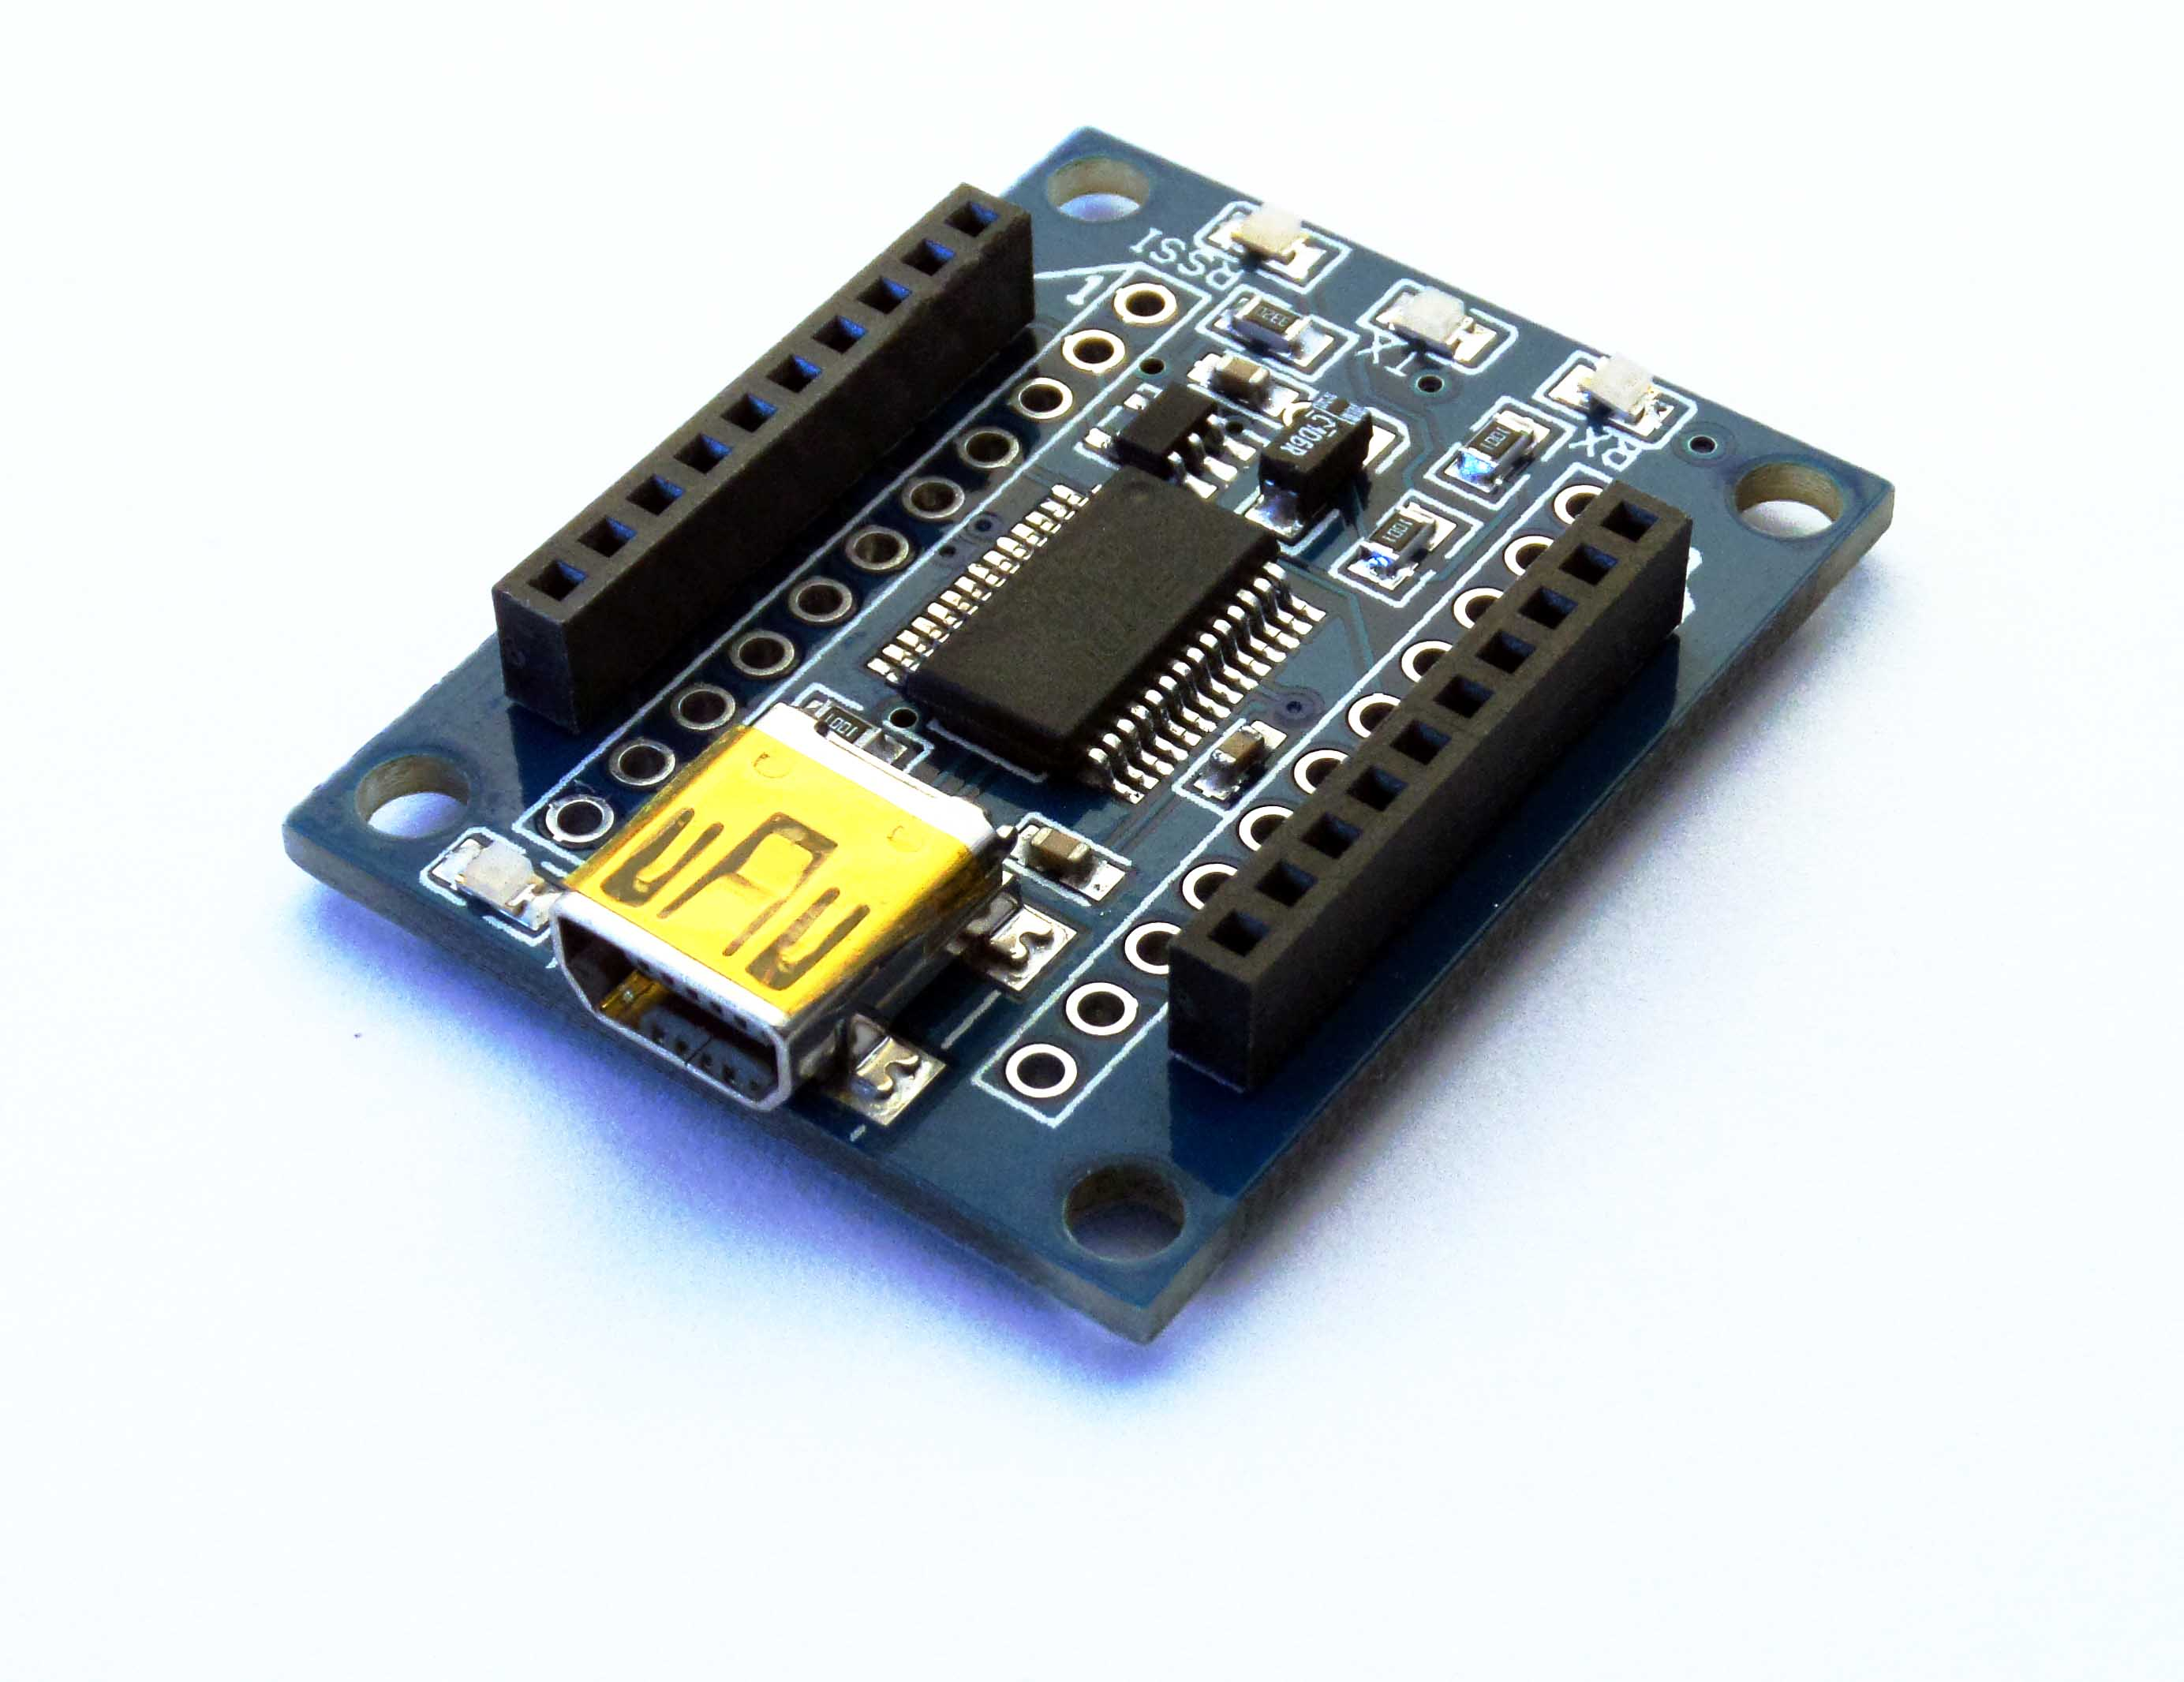
\includegraphics[width=1\textwidth]{./imagenes/xbeeexplorer}
\caption{XBee USB Explorer. Imagen extraída de \scriptsize{http://xbee.cl/xbee-explorer-usb/}} \label{fig:xbeeexplorer}
\end{figure}


En la ventana principal tenemos tres secciones: a la izquierda, la lista de los dispositivos
que tenemos conectados a nuestro ordenador; a la derecha, un panel de administración que variará
en función de lo que estemos haciendo con la mota; y arriba, las opciones relacionadas con el descubrimiento
de nuevos dispositivos (izquierda) o distintas acciones sobre la mota (derecha). Podemos verlo en la figura \ref{fig:interfaz1}.\\

\begin{figure}[htb]
\centering
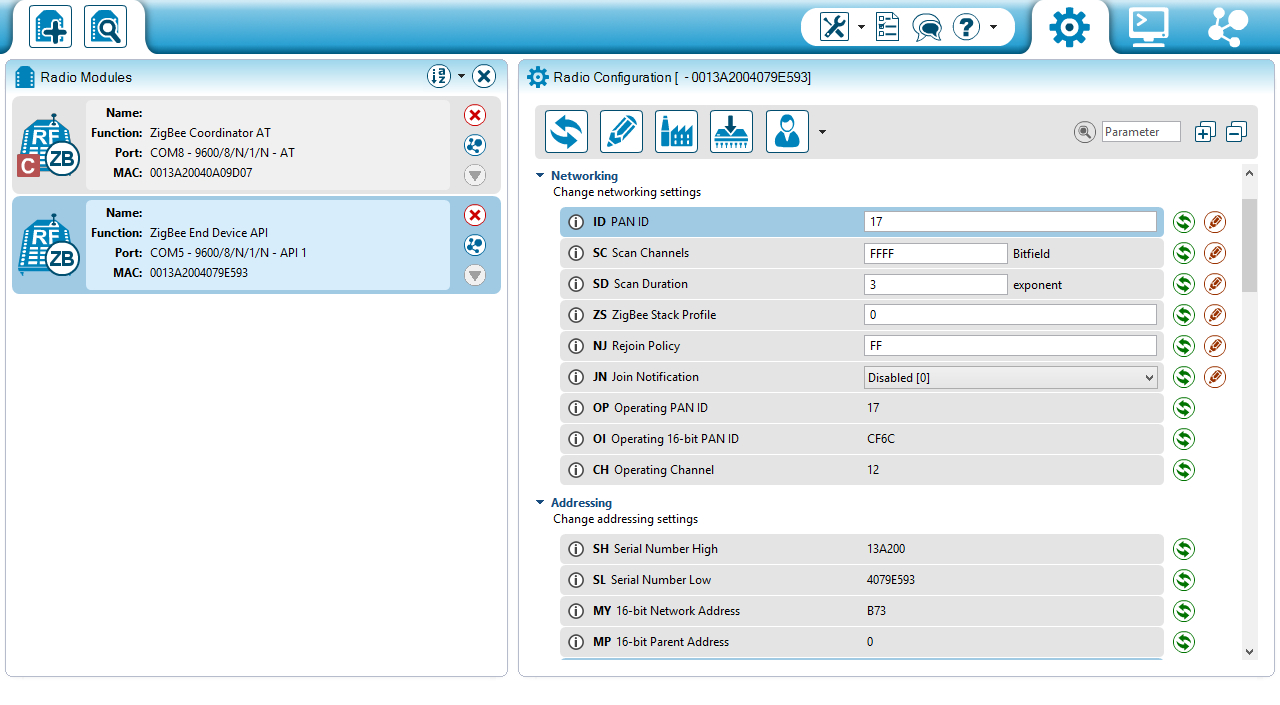
\includegraphics[width=1\textwidth]{./imagenes/interfaz1}
\caption{Interfaz XCTU} \label{fig:interfaz1}
\end{figure}

Lo primero que tendremos que hacer una vez hayamos conectado nuestra mota al ordenador, será descubrirla con XCTU
utilizando una de las dos opciones que tenemos arriba a la izquierda (es importante mencionar que, en caso que se nos
pida resetear la mota y, como es el caso de nuestro modelo, no tengamos un botón para resetear, deberemos unir con un
cable la patilla \guillemotleft RST\guillemotright con \guillemotleft GND\guillemotright).\\

Una vez que tengamos la mota descubierta tendremos el menú de configuración (el de la rueda dentada) abierto. En él podremos
cambiar el firmware, volver a los ajustes de fábrica, establecer un nombre para la mota, ver la dirección de destino,
\textit{PAN} (Personal Area Network) a la que unirse... en función del firmware que tenga instalado la mota, habrá unas opciones u otras
(por ejemplo, en caso de tener un dispositivo final, podremos configurar cada cuánto tiempo de inactividad puede el nodo
entrar en suspensión).\\

En el siguiente menú, podremos ver qué es lo que está recibiendo (o enviando) nuestro XBee. Se monitoriza el puerto serial (ver figura \ref{fig:interfaz2}).\\

\begin{figure}[!htb]
\centering
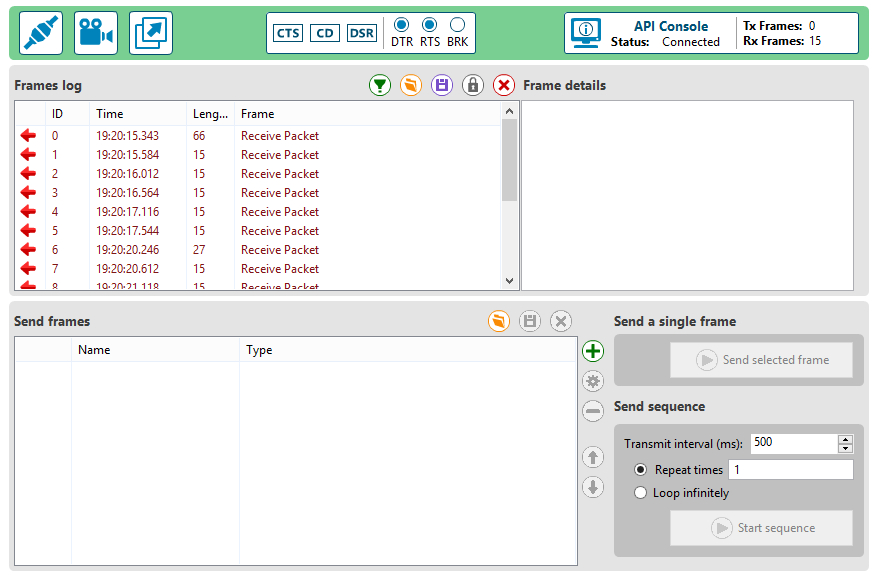
\includegraphics[width=1\textwidth]{./imagenes/interfaz2}
\caption{Monitorizando el puerto serial (modo API) en XCTU} \label{fig:interfaz2}
\end{figure}

Finalmente el tercer menú nos brinda algunas opciones relacionadas con la nube de Digi y la posibilidad
de conocer qué nodos están interconectados en la red (solo disponible si el módulo está en modo API).\\

\subsection{Posible problema de escalabilidad}
\title{Posible problema de escalabilidad}

Aunque estas redes están pensadas para contar con miles de dispositivos,
estas suelen estar formadas por un coordinador y varios routers.
Al haber solamente un coordinador, es éste quien debe almacenar
toda la información que concierne a la red.\\

La dirección MAC de una mota se divide en dos partes iguales (dirección alta y dirección baja).
Teniendo en cuenta que la MAC tiene un tamaño de 64 bits, cada parte tiene un total de 32 bits.
La dirección alta es la misma para todos los nodos y la baja es la que cambia. Por tanto, tendremos 2\textsuperscript{32} direcciones
disponibles (más de 4.000.000.000) o lo que es lo mismo, podremos direccionar hasta 2\textsuperscript{32} dispositivos.\\

El problema que se presenta es el siguiente: Cada dirección ocupa 64 bits, osea, 8 bytes. Si deseamos guardar 150
direcciones (en la introducción se hablaba de casos en los que había bandas que superan los 100 integrantes por lo que
deberíamos pensar en guardar un número mayor de direcciones, donde cada dirección sería un músico), tendremos que almacenar
1.200 bytes (8 bytes x 150 direcciones), unos 1.17KB. Si la memoria destinada a direcciones en la mota es menor que este tamaño,
pueden producirse problemas.\\

Ya que no se disponen de tantos dispositivos para hacer un experimento ni se ha encontrado información al respecto,
no podemos predecir el comportamiento del sistema ante tal número de nodos.\\

\section{Controlador}
\title{Controlador}

Para llevar a cabo el control de los componentes es necesario algún tipo de microcontrolador
o placa controladora. Se han estudiado dos posibles soluciones:

\begin{description}
  \item[PIC] \hfill \\
    \begin{itemize}
      \item Son microcontroladores
      \item Precio muy bajo
      \item Gran variedad
      \item Pequeño tamaño
      \item Programación en ensamblador, con una media de 35 instrucciones
      \item Simples pero orientados a un público muy relacionado con la programación
    \end{itemize}
    \begin{figure}[htb]
    \centering
    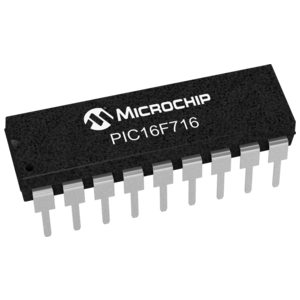
\includegraphics[width=0.6\textwidth]{./imagenes/pic}
    \caption{PICPIC16F716. Imagen extraída de \scriptsize{http://www.microchip.com/}} \label{fig:pic}
    \end{figure}
  \item[Arduino] \hfill \\
    \begin{itemize}
      \item Placa con un microcontrolador
      \item Programación en alto nivel (Python, Scratch, JavaScript o un derivado de Processing)
      \item Muchas bibliotecas para extender funcionalidad
      \item Existe una versión Wear (Arduino Lilypad, mostrado en la figura \ref{fig:lilypad})
      \item Shields para XBee (como la que se muestra en la figura \ref{fig:lilypadxbee})
    \end{itemize}
    \begin{figure}[htb]
    \centering
    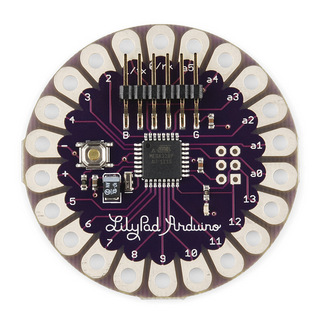
\includegraphics[width=0.6\textwidth]{./imagenes/lilypad}
    \caption{PICPIC16F716. Imagen extraída de \scriptsize{https://www.arduino.cc}} \label{fig:lilypad}
    \end{figure}
    \begin{figure}[htb]
    \centering
    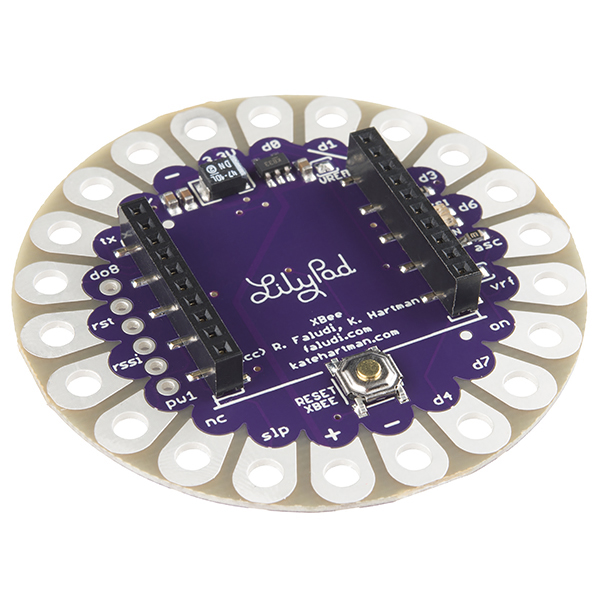
\includegraphics[width=0.6\textwidth]{./imagenes/lilypadxbee}
    \caption{Shield XBee Lilypad. Imagen extraída de \scriptsize{https://www.faludi.com/ \cite{faludi}}} \label{fig:lilypadxbee}
    \end{figure}
\end{description}


\clearpage

Aunque las posibilidades con PIC son mayores, tenemos que tener en cuenta que se desea que la
plataforma atraiga a un número de desarrolladores. Sabiendo que Arduino se encuentra orientado a un
público con una menor formación en electrónica y programación (por lo tanto, accesible a una mayor comunidad), se
adecua más al objetivo de este proyecto. También hay que tener en cuenta la cantidad de bibliotecas
existentes en Arduino (lo que nos ayudará a abstraernos de algunas tareas). Los problemas a los que
nos enfrentamos al elegir esta plataforma son el precio y el tamaño (ambos superiores en Arduino).\\



\section{Alimentación}
\title{Alimentación}

Gracias a la existencia de distintos tipos de placas Arduino, podemos crear dispositivos
con una forma u otra (como otro de los objetivos es la posibilidad de aumentar la funcionalidad
el sistema, habrá funcionalidades que necesiten de placas Arduino con un número distinto de
entradas/salidas al que se utilice aquí), aunque tendremos que intentar que sea lo más compacto
posible (para no ignorar aquel objetivo en el que se deseaba crear un sistema pequeño y discreto).\\

Por ejemplo, en caso que nos encontremos utilizando un Arduino Lilypad, la versión vestible de Arduino,
podremos elegir alguna de las opciones que se nos brindan para alimentar nuestro circuito, como el “LLYP-PSU”,
en el que podremos colocar una pila AAA o el “LilyPad 20mm Coin Cell Battery Holder”, para pilas de botón (cuyos
planos se encuentran disponibles en GitHub \cite{lilypadcoin}).\\

Otra opción a contemplar (y que cobrará mayor sentido al no usar la versión de Arduino vestible)
es la de utilizar bancos de energía (baterías externas). Estas baterías están pensadas para cargar
dispositivos móviles con gran consumo energético. La alta capacidad de estas baterías y el bajo consumo
de Arduino y XBee, tendrá como resultado la despreocupación del usuario en cuanto al plano energético.\\

Como se ha mencionado, en función del tipo de Arduino con el que construyamos nuestro ArduBand,
se seleccionará un tipo de alimentación u otra, quedando esto, generalmente, a opción del usuario
(sobre todo en el caso de la batería externa).\\
